\chapter{Optimierung - Mathematische Grundlagen und Methoden}\label{cha:Optimierung}
In diesem Kapitel werden die notwendigen mathematischen Grundlagen beschrieben, die zur Formulierung eines \gls{OP} und zu dessen Lösung mithilfe der Variationsrechnung notwendig sind. Dazu wird zunächst der Unterschied zwischen \textit{statischer} und \textit{dynamischer} Optimierung erläutert und anschließend mit der \textit{Variationsrechnung} eine Lösungsmethode eingeführt, durch die sich ein dynamisches \gls{OP} in ein System nichtlinearer \gls{DGL} 1. Ordnung überführen lässt. Dessen Lösung kann entweder analytisch oder numerisch bestimmt werden. Danach werden zusätzliche Methoden erläutert, mit deren Hilfe sich ein komplexes \gls{OP} in mehrere miteinander verknüpfte Optimierungsaufgaben unterteilen lässt, deren Lösungen vergleichsweise einfach bestimmt werden können. Abschließend werden einige Lösungsverfahren zur numerischen Lösung dynamischer \gls{OP} vorgestellt und diskutiert. 
\section{Statische Optimierung}\label{sec:statischeOpt}
Die allgemeine Standardformulierung eines statischen \gls{OP} lautet \cite{KnutGraichen.2012}:
\begin{align}
	\min_{\ve{x}\in\mathbb{R}^n} \quad &\fofx \label{eq:J_statisch}\\
	\textrm{u.B.v.} \quad&\mathbf{g}(\ve{x}) = \ve{0} \label{eq:GNB_statisch}\\
	&\mathbf{h}(\ve{x}) \leq \ve{0} \label{eq:UNB_statisch}
\end{align}
Die Funktion \fofx~wird dabei als Kosten- oder Gütefunktion bezeichnet und bezüglich der Optimierungsvariablen $\ve{x}$ unter Berücksichtigung der Nebenbedingungen $\ve{g}$ und $\ve{h}$ minimiert. Bei der statischen Optimierung sind die Variablen $\ve{x}$ Elemente des Euklidischen Raums \cite{KnutGraichen.2012}. Für die \gls{GNB} $\ve{g}(\ve{x})$ und die \gls{UNB} $\ve{h}(\ve{x})$ gilt $\ve{g}\in\mathbb{R}^p$ bzw. $\ve{h}\in\mathbb{R}^q$, wobei $p<n$ sein muss, da sich die Optimierungsvariablen $\ve{x}$ ansonsten bei $p=n$ unabhängigen Gleichungen direkt aus $\mathbf{g}(\ve{x})$ bestimmen lassen \cite{Papageorgiou.2012}. Für die Dimension der \gls{UNB} hingegen gibt es keine maximal zulässige Anzahl \cite{Papageorgiou.2012}.
\section{Dynamische Optimierung}\label{sec:dynamischeOpt}
Im Unterschied zur statischen Optimierung sind die Optimierungsvariablen bei der dynamischen Optimierung selbst Funktionen einer unabhängigen Variable, welche in den meisten Fällen der Zeit $t$ entspricht \cite{KnutGraichen.2012}. Das bedeutet, es werden die optimalen Zeitverläufe der Optimierungsvariablen gesucht. Aufgrund dessen wird die zu optimierende Funktion \fofx~zum Kosten- oder Gütefunktional \J, welches bei der dynamischen Optimierung minimiert wird. Eine sehr häufige Anwendung der dynamischen Optimierung findet man bei dynamischen Systemen, für die eine optimale Eingangstrajektorie \uoptoft~gesucht wird \cite{KnutGraichen.2012}. Da es sich bei den Optimierungsvariablen um die Eingangs- bzw. Steuergrößen des Systems handelt, wird auch von einem \textit{Optimalsteuerungsproblem} gesprochen \cite{KnutGraichen.2012}. Gleichzeitig liefert die Lösung des Problems die optimalen Zustandstrajektorien \xoptoft, weshalb die Formulierung eines dynamischen \gls{OP} einen geeigneten Ansatz zur Trajektorienplanung dynamischer Systeme darstellt. 
Die allgemeine Formulierung eines solchen Optimalsteuerungsproblems lautet \cite{KnutGraichen.2012}:
\begin{align}
\min_{\uoft} \quad &J(\xoft,\uoft,t,t_f) = \Vofxoftf + \int_{t_0}^{t_f}l(\xoft,\uoft,t)~\dtint{t} \label{eq:J_dyn}\\
\textrm{u.B.v.} \quad& \dxoft = \ve{f}(\xoft,\uoft,t)\,,\qquad \xoftzero = \xzero \label{eq:system_anfang}\\
&\mathbf{g}(\xoftf,t_f) = 0 \label{eq:GNB}\\
&\mathbf{h}(\xoft,\uoft) \leq 0\,,\quad \forall t \in [t_0, t_f] \label{eq:UNB}
\end{align}
Es gilt $\ve{x}\in\mathbb{R}^n, \ve{u}\in\mathbb{R}^m, \mathbf{g}\in\mathbb{R}^p$ und $\mathbf{h}\in\mathbb{R}^q$. Wie bereits bei der statischen Optimierung stellen die Gleichungen \eqref{eq:GNB} und \eqref{eq:UNB} \gls{GNB} und \gls{UNB} dar, wobei die \gls{UNB} an dieser Stelle lediglich der Vollständigkeit halber in der allgemeinen Form mit angegeben sind. Für die weiteren Betrachtungen -- die Anwendung der Variationsrechnung und die Ergebnisse dieser Arbeit -- werden die \gls{UNB} vernachlässigt, da die Berücksichtigung von \gls{UNB} eine analytische Lösung des \gls{OP} deutlich komplizierter macht. Es sei allerdings darauf hingewiesen, dass sich auch Optimalsteuerungsprobleme mit \gls{UNB} mithilfe des Ansatzes der Variationsrechnung lösen lassen. Für weitere Informationen zum Umgang mit allgemeinen \gls{UNB} für die Systemzustände und/oder Eingangsgrößen sei auf entsprechende Fachliteratur zum Thema Optimierung verwiesen (siehe \cite{Papageorgiou.2012, Gerdts.2010}). 

Gleichung \eqref{eq:system_anfang} beschreibt die Systemdynamik mit der Eingangsgröße \uoft~und den Anfangszuständen \xzero~des Systems, die als Anfangsbedingungen für den Startpunkt $t_0$ fungieren. Gleichung \eqref{eq:GNB} stellt dabei Endbedingungen für den Endpunkt $t_f$ dar. Gemeinsam bilden die Anfangs- und Endbedingungen die Randbedingungen des Optimierungsproblems. Die dargestellte Form von Randbedingungen wird auch als separierte Randbedingungen bezeichnet, da sich die Bedingungen für den Anfangspunkt und den Endpunkt getrennt voneinander formulieren lassen und keine Randbedingungen der Form $\ve{g}(\xoftzero,\xoftf)=0$ existieren, die gleichzeitig von \xoftzero~und \xoftf~abhängen \cite{Cash.1980}. Das Gütefunktional in Gleichung \eqref{eq:J_dyn} wird in der dargestellten Form auch als \textit{Bolza-Form} des Gütefunktionals bezeichnet und setzt sich aus zwei Teilen zusammen: Der Integralanteil beschreibt die von der Zeit abhängigen laufenden Kosten und heißt \textit{Lagrange-Form}. Der vor dem Integralanteil stehende Term \Vofxoftf~gibt die Bewertung des Endzustands (und der Endzeit), also die Endkosten, an. Dieser wird \textit{Mayer-Form} genannt \cite{KnutGraichen.2012}. Für die Lagrange- und Bolza-Form gilt, dass sie sich immer in die Mayer-Form überführen lassen \cite{KnutGraichen.2012} (siehe auch \cite{Gerdts.2010}). Der Endzeitpunkt $t_f$ kann festgelegt sein oder frei. Ist er frei, so muss $t_f$ als zusätzliche Optimierungsvariable bei der Lösung des \gls{OP} berücksichtigt werden \cite{KnutGraichen.2012}. Häufig hängt das Gütefunktional von mehreren Größen ab, die miteinander konkurrieren können. So steht beispielsweise eine geringe Fahrzeugbeschleunigung im Widerspruch zu einer kurzen Reisezeit. Dies führt dazu, dass bei der Optimierung immer der bestmögliche Kompromiss zwischen allen berücksichtigten Gütekriterien gesucht wird. Beim Optimum eines \gls{OP} wird daher auch von \textit{Pareto-Optimalität} gesprochen \cite{Papageorgiou.2012}. Das Optimum besitzt dann die Eigenschaft, dass die Verbesserung bezüglich eines Gütekriteriums nur auf Kosten der Verschlechterung eines anderen Kriteriums möglich ist -- eine Verbesserung aller Gütekriterien ist nicht möglich \cite{Papageorgiou.2012}. Dies hat zur Folge, dass zum einen die einzelnen Gütekriterien isoliert betrachtet nie ihren bestmöglichen Wert erreichen. Zum anderen hilft diese Eigenschaft dabei, sinnvolle Problemstellungen zu formulieren. Welches der einzelnen Gütekriterien letztendlich wie stark gewichtet wird, unterliegt oftmals der subjektiven Beurteilung. Dadurch kann ein Optimum subjektiv betrachtet \glqq besser\grqq~sein als ein anderes, obwohl beide die Lösung der jeweiligen Problemstellung liefern. Um die Bedeutung von Gütekriterien und Gewichtung zu verdeutlichen, ist in \eqref{eq:Bsp_Gütefunktional} beispielhaft ein einfaches Gütefunktional dargestellt, welches für die Trajektorienplanung im Kontext \gls{AD} verwendet werden könnte 
\begin{equation}
J(a_x,t,t_f) = w_t t_f + \int_{t_0}^{t_f}w_a a_x^2~\dtint{t}\,. \label{eq:Bsp_Gütefunktional}
\end{equation}
Das Gütefunktional setzt sich im dargestellten Fall aus den beiden Gütekriterien Endzeitpunkt $t_f$ und dem Integral über der Längsbeschleunigung $a_x$ zusammen. Das Optimierungsziel dieses Gütefunktionals besteht also darin, eine möglichst geringe Endzeit zu erreichen, und gleichzeitig die laufenden Kosten durch die Beschleunigung zu minimieren -- zwei Ziele, die offensichtlich miteinander konkurrieren. Wie stark die beiden Gütekriterien jeweils in die Bewertung einfließen, lässt sich über die Wahl der Gewichtungsfaktoren $w_t$ und $w_a$ festlegen. Eine höhere Gewichtung führt dazu, dass die jeweilige Größe an Einfluss gewinnt und der Fokus bei der Minimierung mehr auf die entsprechende Größe gelegt wird. Wird beispielsweise die Gewichtung der Beschleunigung $w_a$ erhöht, während $w_t$ unverändert bleibt, führt dies zu einem insgesamt niedrigeren Beschleunigungsniveau und gleichzeitig zu einer längeren Endzeit $t_f$.
\subsection{Variationsrechnung}\label{subsec:Variationsrechnung}
Die Variationsrechnung bietet einen Ansatz, mit dem dynamische \gls{OP} der Gleichungen \eqref{eq:J_dyn}--\eqref{eq:UNB} gelöst werden können. Dazu werden ausgehend von den optimalen Trajektorien \xoptoft~und \uoptoft~und dem optimalen Endzeitpunkt \opt{t_f} (sofern $t_f$ frei und damit Teil der Optimierung ist) Variationen zugelassen, sodass gilt \cite{KnutGraichen.2012}:
\begin{align}
\xoft &= \xoptoft + \epsilon\variation{x}(t) \label{eq:x_var}\\
\dxoft &= \dxoptoft + \epsilon\variation{\dot{x}}(t) \label{eq:dx_var}\\
\uoft &= \uoptoft + \epsilon\variation{u}(t) \label{eq:u_var}\\
t_f &= \opt{t_f} + \epsilon\delta_{t_f}\label{eq:t_var}
\end{align}
Die $\ve{\delta}$-Variablen bezeichnen dabei die Variationen der einzelnen Größen und $\epsilon$ ist der Parameter, mit dem die Variationen Einfluss auf die Trajektorien nehmen, wobei für $\epsilon=0$ offensichtlich $\xoft=\xoptoft$, $\dxoft = \dxoptoft$, $\uoft=\uoptoft$ und $t_f=\opt{t_f}$ gilt. In Abbildung \ref{fig:Variation} ist ein solcher Verlauf einer möglichen optimalen Trajektorie \xoptoft~und einer zulässigen Variation skizziert. Außerdem sind die Variation des Endzeitpunkts und des Endzustands $\xoftf = \xoptoftfopt+\epsilon(\variation{x}(\opt{t_f})+\dxoptoftfopt\delta_{t_f})$ dargestellt.
\begin{figure}[h]
\centering
\begin{tikzpicture}[scale=1.5, domain=0:4, samples=200]
\draw[->] (0,0) -- (5,0) node[right] {$t$};
\draw[->] (0,0) -- (0,4) node[above] {$x$};
\draw[color=black,domain=0:4,-*]    plot (\x,{sqrt(\x)});
\draw[color=mycolor,domain=0:4,-]   plot (\x,{sqrt(\x)+0.5*sin(3*\x r)});
\draw[color=mycolor,domain=4:4.5,-*]   plot (\x,1.3*\x-3.468286);
\draw [dashed] (3.95,0) node[below] {$\opt{t_f}$} -- (3.95,3);
\draw [dashed] (4.45,0) node[below] {$t_f$} -- (4.45,3);
\draw[-] (4.45,2.5) -- (4.8,2.5);
\draw[-] (3.95,2) -- (4.8,2);
\draw [stealth-stealth] (3.95,0.7) -- (4.45,0.7) node[midway,above] {$\delta_{t_f}$};
\draw [stealth-stealth] (4.7,2) -- (4.7,2.5) node[midway,right] {$\variation{x}(\opt{t_f})+\dxoptoftfopt\delta_{t_f}$};
\draw [-stealth] (2.7,0.7) node[below] {$\xoptoft + \epsilon\variation{x}(t)$} -- (3.3,1.4) ;
\draw [-stealth] (1.3,2) node[above] {\xoptoft} -- (1.5,1.3) ;
\draw [-stealth] (3.2,2.5) node[above] {$\xoptoftfopt$} -- (3.8,2.1) ;
\end{tikzpicture}
\caption{Schematische Darstellung der optimalen Trajektorie \xoptoft~und eine mögliche, zulässige Variation \xoft nach \cite{KnutGraichen.2012}.}
\label{fig:Variation}
\end{figure}

Für die Anwendung der Variationsrechnung zur Optimierung dynamischer Systeme wird das folgende Gütefunktional definiert \cite{KnutGraichen.2012}:
\begin{equation}
J(\xoft,\dxoft,\uoft,t,t_f) = \Vofxoftf + \int_{t_0}^{t_f}l(\xoft,\uoft,t) + \lambdaoft^T(\ve{f}(\xoft,\uoft,t) - \dxoft)~\dtint{t} \label{eq:J_var_sys}
\end{equation}
Im Vergleich zur Formulierung in \eqref{eq:J_dyn} wurde der Lagrange-Teil des Gütefunktionals im Integral um den Term $\int\lambdaoft^T(\ve{f}(\xoft,\uoft,t) - \dxoft)$ erweitert, wobei dieser für $\dxoft = \ve{f}(\xoft,\uoft,t)$ zu null wird. Die Variablen $\ve{\lambda}\in\mathbb{R}^n$ stellen dabei die sogenannten \textit{adjungierten Zustände} dar \cite{KnutGraichen.2012}. Durch das Einführen dieser Multiplikatoren ist es möglich, die in \eqref{eq:system_anfang} als Nebenbedingung formulierte Systemdynamik in das Gütefunktional hineinzuziehen \cite{Follinger.1994}. Werden die Variablen im Gütefunktional nun durch die Gleichungen \eqref{eq:x_var}--\eqref{eq:t_var} ersetzt, hängt das Gütefunktional nur noch von $\epsilon$ ab. Da die Trajektorien \xoft, \dxoft~und \uoft~wie bereits gezeigt nur für $\epsilon=0$ den optimalen Verläufen entsprechen können, lautet die notwendige Bedingung für das Verschwinden der Variation des Gütefunktionals $\delta_J$ und damit für ein Minimum 
\begin{equation}
	\delta_J = \frac{\textrm{d}J(\xoptoft+\epsilon\variation{x}(t),\dxoptoft + \epsilon\variation{\dot{x}}(t),\uoptoft + \epsilon\variation{u}(t),\opt{t_f} + \epsilon\delta_{t_f})}{\dtint{\epsilon}}\Big|_{\epsilon=0}=0\,. \label{eq:VariationJ}
\end{equation}
Aus dieser Bedingung lassen sich die notwendigen Optimalitätsbedingungen für eine optimale Lösung herleiten. Aus Gründen der Übersichtlichkeit wird nachfolgend auf die explizite Nennung aller Argumente verzichtet, dort wo diese nicht unbedingt notwendig sind. Die Differentiation des Gütefunktionals liefert nach \cite{KnutGraichen.2012} die totale Variation 
\begin{equation}
\begin{split}
\delta_J &=  \Big(\Big(\frac{\partial V}{\partial \ve{x}}\Big)^T - \ve{\lambda}^T\Big)\Big|_{t=t_f}(\variation{x}(\opt{t_f})+\dxoptoftfopt\delta_{t_f}) + \Big(\frac{\partial V}{\partial t} + l + \ve{\lambda}^T\ve{f}\Big)\Big|_{t=t_f}\delta_{t_f} \\
& \qquad + \int_{t_0}^{t_f} \Big(\frac{\partial l}{\partial \ve{x}} + \Big(\frac{\partial \ve{f}}{\partial \ve{x}}\Big)^T \ve{\lambda} + \dot{\ve{\lambda}}\Big)^T \variation{x} + \Big(\frac{\partial l}{\partial \ve{u}} + \Big(\frac{\partial \ve{f}}{\partial \ve{u}}\Big)^T \ve{\lambda}\Big)^T \variation{u} ~\dtint{t}\,, \label{eq:J_totale_Variation}
\end{split}
\end{equation}
aus der sich die nachfolgenden Optimalitätsbedingungen ableiten lassen. Auf die vollständige Herleitung von Gleichung \eqref{eq:J_totale_Variation} wurde an dieser Stelle verzichtet und es sei für den gesamten Rechenweg auf weiterführende Literatur verwiesen \cite{KnutGraichen.2012,Papageorgiou.2012,Gerdts.2010}.
\subsubsection{Optimalitätsbedingungen}\label{subsubsec:Optimalitätsbedingungen}
Bevor die Optimalitätsbedingungen aus Gleichung \eqref{eq:J_totale_Variation} angegeben werden, wird zunächst die \textit{Hamilton-Funktion} als 
\begin{equation}
	H(\xoft,\uoft,\lambdaoft,t) = l(\xoft,\uoft,t) + \lambdaoft^T\ve{f}(\xoft,\uoft,t) \label{eq:Hamilton}
\end{equation}
definiert, mit deren Hilfe die Optimalitätsbedingungen angegeben werden können. Damit die notwendige Bedingung für ein Minimum \eqref{eq:VariationJ} erfüllt sein kann, müssen nach \cite{KnutGraichen.2012} die folgenden Optimalitätsbedingungen erfüllt sein 
\begin{alignat}{2}
	\dx &= \frac{\partial H}{\partial\ve{\lambda}} & &= \ve{f}(\ve{x},\ve{u},t) \label{eq:Zustandsdgl} \\
	\dlambda &= -\frac{\partial H}{\partial \ve{x}} & &= -\frac{\partial l}{\partial \ve{x}} - \Big(\frac{\partial \ve{f}}{\partial \ve{x}}\Big)^T \ve{\lambda} \label{eq:Adjdgl} \\
	\ve{0} &= \frac{\partial H}{\partial \ve{u}} & &= \frac{\partial l}{\partial \ve{u}} + \Big(\frac{\partial \ve{f}}{\partial \ve{u}}\Big)^T \ve{\lambda}\,. \label{eq:Steuerungsgleichung} 
\end{alignat}
Diese Bedingungen ergeben sich aus der Ableitung der Hamilton-Funktion nach den adjungierten Zuständen und daraus, dass die einzelnen Summanden im Integral der totalen Variation \eqref{eq:J_totale_Variation} Null ergeben müssen. Gleichung \eqref{eq:Zustandsdgl} beschreibt die Zustandsdifferentialgleichung, während Gleichung \eqref{eq:Adjdgl} die \gls{DGL} für die adjungierten Zustände $\ve{\lambda}$ beschreibt und daher auch \textit{adjungierte \gls{DGL}} genannt wird \cite{Konigorski.2019}. Die beiden Gleichungen \eqref{eq:Zustandsdgl} und \eqref{eq:Adjdgl} werden auch als \textit{kanonische \gls{DGL}} bezeichnet und bilden gemeinsam mit der Steuerungsgleichung \eqref{eq:Steuerungsgleichung} die sogenannten \textit{Hamiltongleichungen} \cite{Konigorski.2019}. Die kanonischen \gls{DGL} lassen sich zu einer gemeinsamen Systemdynamik 
\begin{equation}
	\dz = \begin{bmatrix}
	\dx \\
	\dlambda
	\end{bmatrix} = 
	\begin{bmatrix}
	\ve{f}(\ve{x},\ve{u},t) \\
	-\frac{\partial H}{\partial \ve{x}}
	\end{bmatrix} \label{eq:Sysdyn_z}
\end{equation}
zusammenfassen.
Nach \cite{KnutGraichen.2012} lauten die Randbedingungen für das \gls{OP} 
\begin{alignat}{2}
\xoftzero &= \xzero \label{eq:Anfangswerte} \\
x_i(t_f) &= x_{f,i}\,, & & \quad i \in\mathcal{I}_f \label{eq:Endwerte} \\
\lambda_i(t_f) &= \frac{\partial V}{\partial x_i}\Big|_{t=t_f}\,, & & \quad i \notin \mathcal{I}_f \label{eq:Lambdaend} \\
H(\ve{x},\ve{u},\ve{\lambda},t)\Big|_{t=t_f} &= -\frac{\partial V}{\partial t}\Big|_{t=t_f}\,, & & \quad \textrm{falls, $t_f$ frei ist.} \label{eq:Transversalitaet}
\end{alignat}
Die Gleichungen \eqref{eq:Anfangswerte} und \eqref{eq:Endwerte} geben die Randbedingungen für die Anfangs- und Endwerte der Zustände an. Dabei bezeichnet $\mathcal{I}_f$ die Menge aller Zustände, die explizit über Endbedingungen vorgegeben sind -- eine Vorgabe der Endwerte ist dabei nicht zwingend notwendig. Für solche Zustände, deren Endwert nicht vorgegeben und damit frei ist, gilt Gleichung \eqref{eq:Lambdaend}. Gleichung \eqref{eq:Transversalitaet} gilt nur dann, falls $t_f$ frei und damit eine Optimierungsvariable des Problems ist und gibt so die zusätzliche notwendige Gleichung zur Bestimmung der freien Endzeit an. Die Gleichungen \eqref{eq:Lambdaend} und \eqref{eq:Transversalitaet} werden als \textit{Transversalitätsbedingungen} bezeichnet und folgen daraus, dass auch die Summanden außerhalb des Integrals der totalen Variation \eqref{eq:J_totale_Variation} Null ergeben müssen \cite{KnutGraichen.2012}. 
\subsubsection{Notwendige Bedingung 2. Ordnung}\label{subsubsec:Legendre_Bedingung}
Da die Bedingung \eqref{eq:VariationJ} die erste Variation des Gütefunktionals darstellt, werden die hergeleiteten Optimalitätsbedingungen, die aus \eqref{eq:VariationJ} resultieren, auch als notwendige Optimalitätsbedingungen 1. Ordnung bezeichnet \cite{Papageorgiou.2012}. Diese stellen lediglich notwendige Bedingungen für die Existenz eines Minimums dar, da die Bedingung \eqref{eq:VariationJ} auch für alle anderen Extrema (Maximum, Sattelpunkt) erfüllt ist und daher nicht hinreichend für die Existenz eines Minimums ist \cite{Papageorgiou.2012}. Lösungen, die die Optimalitätsbedingungen erfüllen, sind also zunächst einmal nur Kandidaten für ein Minimum und damit für eine optimale Lösung \cite{Gerdts.2010}. Da die Herleitung hinreichender Optimaliätsbedingungen mit erheblichem Aufwand verbunden ist, sei an dieser Stelle auf weiterführende Literatur zu diesem Thema verwiesen (siehe \cite{Gerdts.2010,Maurer.1981}). Allerdings lässt sich analog zu \eqref{eq:VariationJ} aus der zweiten Variation des Gütefunktionals eine notwendige Optimalitätsbedingung 2. Ordnung herleiten
\begin{equation}
\delta^2_J = \frac{\textrm{d}^2J}{\dtint{\epsilon^2}}\Big|_{\epsilon=0}\geq 0\,,
\end{equation}
welche auch als \textit{Legendre-Bedingung} bekannt ist \cite{KnutGraichen.2012}. Für Optimalsteuerungsprobleme lässt sich die notwendige Optimalitätsbedingung 2. Ordnung für ein schwaches, lokales Minimum mit 
\begin{equation}
\frac{\partial^2 H}{\partial \ve{u}} \quad \textrm{ist positiv semidefinit} \quad \forall t \in[t_0,t_f]
\end{equation}
angeben \cite{KnutGraichen.2012}. Die zweifache, partielle Ableitung beschreibt dabei die Hessematrix der Hamilton-Funktion bezüglich der Stellgrößen. Ein häufig auftretender Fall bei der Optimierung dynamischer Systeme liegt in der Optimierung eingangsaffiner, autonomer Systeme\footnote{Die Klasse der autonomen Systeme beschreibt den Fall, dass der Güteterm $l(\ve{x},\ve{u})$ und die Systemdynamik $\ve{f}(\ve{x},\ve{u})$ nicht explizit, sondern nur implizit über $\ve{x}$ und $\ve{u}$ von der Zeit $t$ abhängen \cite{KnutGraichen.2012}.} mit quadratischer oder linear-quadratischer Bestrafung der Stellgröße. Nachfolgend ist die Anwendung der Legendre-Bedingung für Systeme dieser Klasse gezeigt. Die Eingangsaffinität für ein System mit $m$ Stellgrößen lässt sich allgemein durch 
\begin{equation}
\ve{f}(\ve{x},\ve{u}) = \ve{f}_0(\ve{x})+\ve{f}_1(\ve{x})u_1+\dots+\ve{f}_m(\ve{x})u_m
\end{equation}
ausdrücken und das Gütefunktional lässt sich mit
\begin{equation}
J(\ve{x},\ve{u},t,t_f) = t_f + \int_{t_0}^{t_f} l_0(\ve{x}) + l_1(\ve{x},u_1) + \dots + l_m(\ve{x},u_m)~\dtint{t}
\end{equation}
angeben. Die Hamilton-Funktional ergibt sich damit zu
\begin{equation}
	H(\ve{x},\ve{u},\ve{\lambda},t) = l_0(\ve{x}) + \ve{\lambda}^T\ve{f}_0(\ve{x}) + l_1(\ve{x},u_1) + \ve{\lambda}^T\ve{f}_1(\ve{x})u_1 + \dots + l_m(\ve{x},u_m) + \ve{\lambda}^T\ve{f}_m(\ve{x})u_m \,,
\end{equation}
wobei mit der linear-quadratischen Bestrafung 
\begin{equation}
l_i(\ve{x},u_k) = \tilde{l}_i(\ve{x})u_i^2 + \hat{l}_i(\ve{x})u_i\,, \quad i = 1,2,\dots,m \label{eq:line_quad}
\end{equation}
gilt. Beim Aufstellen der Hessematrix müssen in jedem Eintrag nur die Anteile von $H$ berücksichtigt werden, die explizit von der jeweiligen Stellgröße abhängen. Unter Berücksichtigung von \eqref{eq:line_quad} lautet die Legendre-Bedingung schließlich
\begin{align}
\frac{\partial^2 H}{\partial \ve{u}} &= 
\begin{bmatrix}
\frac{\partial^2 l_1(\ve{x},u_1)}{\partial u_1^2} & 0 &  \dots & 0 \\
0 & \frac{\partial^2 l_2(\ve{x},u_2)}{\partial u_2^2} & \dots & 0 \\
\vdots & \vdots & \ddots & \vdots \\
0 & \dots & 0 & \frac{\partial^2 l_m(\ve{x},u_m)}{\partial u_m^2}
\end{bmatrix} \\
 &= 
\begin{bmatrix}
	2\tilde{l}_1(\ve{x}) & 0 &  \dots & 0 \\
	0 & 2\tilde{l}_2(\ve{x}) & \dots & 0 \\
	\vdots & \vdots & \ddots & \vdots \\
	0 & \dots & 0 & 2\tilde{l}_m(\ve{x})
\end{bmatrix} \quad \textrm{ist positiv semidefinit} \quad \forall t \in[t_0,t_f] \,.
\end{align} 
Diese kann verwendet werden, um die Lösungskandidaten weiter bezüglich Maxima und Minima zu sortieren \cite{Papageorgiou.2012}.
\subsubsection{Singulärer Fall}\label{subsubsec:Singularität}
In der Regel lässt sich die Eingangsgröße aus der Steuerungsgleichung \eqref{eq:Steuerungsgleichung} durch die Systemzustände und die adjungierten Zustände ausdrücken, wobei dies nicht immer der Fall sein muss \cite{KnutGraichen.2012}. Für \gls{OP}, die ein eingangsaffines System optimieren und in denen $l(\ve{x},\ve{u},t)$ unabhängig von $\ve{u}$ ist, gilt 
\begin{equation}
	\frac{\partial H}{\partial \ve{u}} = \frac{\partial (l(\ve{x},t) + \ve{\lambda}^T(\ve{f}_0(\ve{x})+\ve{f}_1(\ve{x})\ve{u}))}{\partial \ve{u}} = \ve{\lambda}^T\ve{f}_1(\ve{x}) \stackrel{!}{=} 0 \,. \label{eq:dhduzero}
\end{equation}
Die Darstellung $\ve{f}(\ve{x},\ve{u},t) = \ve{f}_0(\ve{x})+\ve{f}_1(\ve{x})\ve{u}$ verdeutlicht dabei die Eingangsaffinität des dynamischen Systems. Aus Gleichung \eqref{eq:dhduzero} ist direkt zu erkennen, dass sich die Steuergröße \uoft~in diesem Fall nicht durch die Zustände ausdrücken lässt, weshalb auch von einem \textit{singulären} Problem gesprochen wird \cite{KnutGraichen.2012}. Der singuläre Fall kann allerdings in der Praxis leicht umgangen werden, indem das Quadrat der Stellgröße $\ve{u}^2$ mithilfe von hinreichend kleinen Gewichtungen zum Gütefunktional hinzugefügt wird, sodass der Einfluss auf das Optimierungsergebnis vernachlässigbar gering ist, aber trotzdem $\frac{\partial l(\ve{x},\ve{u},t)}{\partial \ve{u}} \neq 0$ gilt \cite{KnutGraichen.2012}.
\subsubsection{Allgemeine Endbedingungen}\label{subsubsec:Allg_Endbedingungen}
Damit neben der Vorgabe einzelner Endzustände auch allgemeine Endbedingungen, wie in Gleichung \eqref{eq:GNB} dargestellt, berücksichtigt werden können, wird das Gütefunktional in Gleichung \eqref{eq:J_var_sys} wie folgt erweitert. Das Funktional zur Betrachtung allgemeiner Endbedingungen lautet
\begin{equation}
J(\ve{x},\dx,\ve{u},t,t_f) = \underbrace{\Vofxoftf + \ve{\nu}^T\mathbf{g}(\xoftf,t_f)}_{\Vofxoftfallgemein} + \int_{t_0}^{t_f}l(\ve{x},\ve{u},t) + \ve{\lambda}^T(\ve{f}(\ve{x},\ve{u},t) - \dx)~\dtint{t}\,. \label{eq:J_var_sys_allgemein}
\end{equation}
Über die \textit{Lagrange-Multiplikatoren} $\ve{\nu}\in\mathbb{R}^p$ wird dabei die Einhaltung der allgemeinen Endbedingungen gewährleistet. Diese sind im Gegensatz zu den adjungierten Zuständen konstant und keine zeitabhängigen Variablen. Die neuen Transversalitätsbedingungen lauten nach \cite{KnutGraichen.2012}
\begin{alignat}{2}
\lambdaoftf &= \frac{\partial \bar{V}}{\partial \ve{x}}\Big|_{t=t_f} & &= \Big(\frac{\partial V}{\partial \ve{x}} + \Big(\frac{\partial \mathbf{g}}{\partial \ve{x}}\Big)^T\ve{\nu}\Big)\Big|_{t=t_f} \label{eq:Lambdaend_allgemein} \\
H(\ve{x},\ve{u},\ve{\lambda},t)\Big|_{t=t_f} &= - \frac{\partial \bar{V}}{\partial t}\Big|_{t=t_f} & &= -\Big(\frac{\partial V}{\partial t}+\Big(\frac{\partial \mathbf{g}}{\partial t}\Big)^T\ve{\nu}\Big)\Big|_{t=t_f}\,,\quad \textrm{falls, $t_f$ frei ist.} \label{eq:Transversalitaet_allgemein}
\end{alignat}
und anstelle von Gleichung \eqref{eq:Endwerte} gilt Gleichung \eqref{eq:GNB}. Somit erhält man zusammen mit den Anfangswerten in Gleichung \eqref{eq:Anfangswerte} insgesamt $2n+p+1$ Randbedingungen zur Bestimmung der $2n+p+1$ Unbekannten $\ve{x}, \ve{\lambda}, \ve{\nu}$ und $t_f$. Werden anstatt allgemeiner Endbedingungen fixierte Endzustände betrachtet, so entfallen $p$ Gleichungen und die $p$ Unbekannten $\ve{\nu}$ und es gilt nur $\ve{x}, \ve{\lambda}$ und $t_f$ zu bestimmen. Es sei dabei angemerkt, dass die allgemeinen Endbedingungen nicht alle Endzustände betreffen müssen und wie bereits in Abschnitt \ref{subsubsec:Optimalitätsbedingungen} auch in diesem Fall Kombinationen aus fixierten Endzuständen und über allgemeine Endbedingungen vorgegebenen Endzuständen möglich sind. 

Mithilfe der Variationsrechnung lässt sich das ursprüngliche dynamische \gls{OP} \eqref{eq:J_dyn}--\eqref{eq:UNB} in ein \gls{ZPR} überführen, dessen Problematik nun darin besteht, die Lösung der kanonischen \gls{DGL} zu bestimmen und das resultierende Randwertproblem zu lösen. 

\subsubsection{Maximumprinzip von Pontryagin}\label{subsubsec:Maximumprinzip}
Bisher wurde davon ausgegangen, dass die Stellgröße $\ve{u}$ unbeschränkt ist. In diesem Fall liefert die Steuerungsgleichung \eqref{eq:Steuerungsgleichung} die notwendige Bedingung, dafür dass das Optimalsteuerungsproblem bezüglich der Stellgröße ein Minimum besitzt. Ist die Stellgröße hingegen mit $\ve{u}\in\mathcal{U}\subseteq\mathbb{R}^m $ beschränkt, verliert diese Bedingung ihre Gültigkeit, da das Minimum auch auf dem Rand der Lösungsmenge $\mathcal{U}$ liegen kann \cite{KnutGraichen.2012}. In diesem Fall kann das sogenannte \textit{Maximumprinzip von Pontryagin} zur Lösung herangezogen werden. Die neue notwendige Optimalitätsbedingung lautet
\begin{equation}
	H(\ve{x}^*, \ve{u}^*, \ve{\lambda}^*, t^*) = \min_{\ve{u}\in\mathcal{U}} H(\ve{x}^*, \ve{u}, \ve{\lambda}^*, t^*)\,, \label{eq:Maximumprinzip}
\end{equation}
wobei diese Bedingung eine Verallgemeinerung der Steuerungsgleichung \eqref{eq:Steuerungsgleichung} darstellt und der unbeschränkte Fall durch die Bedingung \eqref{eq:Maximumprinzip} ebenfalls abgedeckt ist \cite{KnutGraichen.2012}. Für die häufig vorkommende Systemklasse eingangsaffiner, autonomer Systeme mit quadratischer oder linear-quadratischer Bestrafung der Stellgröße lässt sich das Minimum bezüglich der Stellgröße durch die bisher bekannte Steuerungsgleichung \eqref{eq:Steuerungsgleichung} bestimmen, falls das Minimum innerhalb des zulässigen Lösungsbereichs $\mathcal{U}$ liegt. Falls die Lösung der Steuerungsgleichung außerhalb des zulässigen Bereichs liegt, kann die optimale Stellgröße durch eine Fallunterscheidung bestimmt werden \cite{KnutGraichen.2012}. Dies wird in Kapitel \ref{cha:Modellbildung} am verwendeten Fahrzeugmodell angewendet.

\subsection{Optimalitätsprinzip nach Bellman}\label{subsec:Optimalitätsprinzip}
Mitte der 1950er Jahre formulierte Richard Bellman das sogenannte \textit{Optimalitätsprinzip} \cite{Bellman.1984}, welches bis heute bei der dynamischen Optimierung von großer Bedeutung ist und wichtige Erkenntnisse für die Kombination mehrerer \gls{OP} liefert. Das Optimalitätsprinzip besagt, dass wenn \uoptoft~mit $t\in[t_0, t_f]$ eine optimale Trajektorie ist und das System $\dx = \ve{f}(\ve{x},\ve{u},t)$ optimal vom Anfangszustand \xoftzero~in den Endzustand \xoptoftf~überführt, dann ist \uoptoft~mit $t\in[t_1, t_f],\, t_0\leq t_1\leq t_f$ diejenige optimale Trajektorie, die das System aus dem Zwischenzustand $\opt{\ve{x}}(t_1)$ in den optimalen Endzustand \xoptoftf~überführt. Es lässt sich also sagen, dass wenn \uoptoft~ein System optimal von \xoftzero~nach $\opt{\ve{x}}(t_1)$ bringt, dann muss auch \uoptoft~das System optimal von $\opt{\ve{x}}(t_1)$ nach \xoptoftf~bringen und es kann keine andere optimale Trajektorie als \uoptoft~selbst für diesen Abschnitt geben, sofern \uoptoft~auf dem gesamten Intervall $t\in[t_0, t_f]$ optimal ist. Dadurch ist sichergestellt, dass sich die Lösung eines dynamischen \gls{OP} auf dem Intervall $t\in[t_0, t_f]$ immer durch zwei (oder mehrere) Teillösungen 
\begin{equation}
	\min_{\uoft} \int_{t_0}^{t_f}(\cdot)~\dtint{t} = \min_{\uoft} \int_{t_0}^{t_1}(\cdot)~\dtint{t} + \min_{\uoft} \int_{t_1}^{t_f}(\cdot)~\dtint{t}
\end{equation}
angeben lässt. Diese Erkenntnis wird an späterer Stelle in dieser Arbeit (Kapitel \ref{cha:Ergebnisse}) besonders wichtig, wenn es darum geht, die Gesamtlösung eines Verkehrsszenarios anzugeben, welches sich aus mehreren Teilszenarien zusammensetzt. So lässt sich beispielsweise ein Abbiegemanöver durch die Kombination einer vorangestellen Geraden, einer Kurve und anschließend einer zweiten Geraden beschreiben -- dementsprechend setzt sich nach dem Optimalitätsprinzip die Gesamtlösung aus den einzelnen Teillösungen zusammen.
\section{Zeittransformation für freie Endzeitpunkte}\label{sec:Zeittransformation}
Wie bereits gezeigt wurde, kann der Endzeitpunkt $t_f$ frei sein und wird damit ebenfalls zu einer Optimierungsvariable. Dadurch, dass $t_f$ nicht festgelegt ist, ist auch die obere Integrationsgrenze des Gütefunktionals nicht festgelegt. Bei der analytischen Lösung des resultierenden \gls{ZPR} -- sofern sich diese bestimmen lässt -- ist dies nicht weiter kritisch, da $t_f$ mithilfe der Randbedingungen \eqref{eq:Anfangswerte}--\eqref{eq:Transversalitaet} bestimmt werden kann. Bei der Lösung mittels numerischer Lösungsverfahren hingegen kann dies problematisch sein, da viele Lösungsverfahren ein fest definiertes Zeitintervall für die Berechnung der Lösung benötigen (siehe Abschnitt \ref{sec:Lösungsverfahren}), sodass eine alternative Formulierung für die freie Endzeit $t_f$ angegeben werden muss. Dazu bietet es sich an, eine Zeittransformation $\Ttransoftau: [\tau_0, \tau_f] \rightarrow [t_0, t_f]$ einzuführen, die ein festes Zeitintervall $[\tau_0, \tau_f]$ auf die freien Intervallgrenzen $[t_0, t_f]$ abbildet \cite{Gerdts.2010}, wobei 
\begin{align}
	\Ttransoftauzero &= t_0 = \tau_0 = 0 \qquad \textrm{und} \\
	\Ttransoftauf &= t_f
\end{align}
gelten soll. Die festen Intervallgrenzen $[\tau_0, \tau_f]$ können beliebig gewählt werden und eine Wahl von $[\tau_0, \tau_f] = [0, 1]$ stellt dabei keine Einschränkung der Allgemeinheit dar. Eine geeignete Transformation, die diese Kriterien erfüllt lautet
\begin{equation}
	\Ttransoftau = \gamma\tau = t\,, \label{eq:Zeittransformation}
\end{equation}
wobei der \textit{Zeitstreckfaktor} $\gamma$ die anstelle von $t_f$ verwendete neue Optimierungsvariable darstellt \cite{KnutGraichen.2012}. Für die Zeittransformation gilt 
\begin{equation}
	\dTtransoftau = \frac{\partial\Ttransoftau}{\partial\tau} = \frac{\partial t}{\partial\tau} = \gamma\,.
\end{equation}
Bei der Herleitung der Optimalitätsbedingungen unter Verwendung der Zeittransformation muss in den Gleichungen \eqref{eq:J_var_sys}--\eqref{eq:Hamilton} die Substitution \eqref{eq:Zeittransformation} angewendet werden. Außerdem gilt $\partial t = \gamma\partial\tau$ bzw. $\dtint{t} = \gamma\dtint{\tau}$. Dadurch ergeben sich in der transformierten $\tau$-Domäne leicht geänderte Gleichungen. Für die kanonischen \gls{DGL} gilt 
\begin{align}
\dxoftau &= \dTtransoftau\frac{\partial H}{\partial\ve{\lambda}} = \dTtransoftau\ve{f}(\xoftau,\uoftau,\tau) \label{eq:Zustandsdgl_tau} \\
\dlambdaoftau &= -\dTtransoftau\frac{\partial H}{\partial \ve{x}}\,, \label{eq:Adjdgl_tau} 
\end{align}
sodass sich die transformierte gemeinsame Systemdynamik aus Gleichung \eqref{eq:Sysdyn_z} zu 
\begin{equation}
	\dzoftau = \begin{bmatrix}
	\dxoftau \\
	\dlambdaoftau
	\end{bmatrix} = \dTtransoftau
	\begin{bmatrix}
	\ve{f}(\xoftau,\uoftau,\tau) \\
	-\frac{\partial H}{\partial \ve{x}}
	\end{bmatrix} = 
	\gamma
	\begin{bmatrix}
	\ve{f}(\xoftau,\uoftau,\tau) \\
	-\frac{\partial H}{\partial \ve{x}}
	\end{bmatrix} \label{eq:Sysdyn_z_tau}
\end{equation} 
ergibt. Die Randbedingungen bleiben bis auf die Substitution \eqref{eq:Zeittransformation} unverändert. Für eine ausführliche Herleitung der Optimalitätsbedingungen unter Verwendung einer Zeittransformation sei auf \cite{Gerdts.2010} verwiesen.

Bisher wurde die Zeittransformation für ein einzelnes Zeitintervall betrachtet. Diese lässt sich auf $k$ miteinander verknüpfte Intervalle erweitern. In Abbildung \ref{fig:Zeittransformation} ist eine solche Transformation mehrerer gekoppelter Intervalle dargestellt.
\begin{figure}[t]
	\centering
	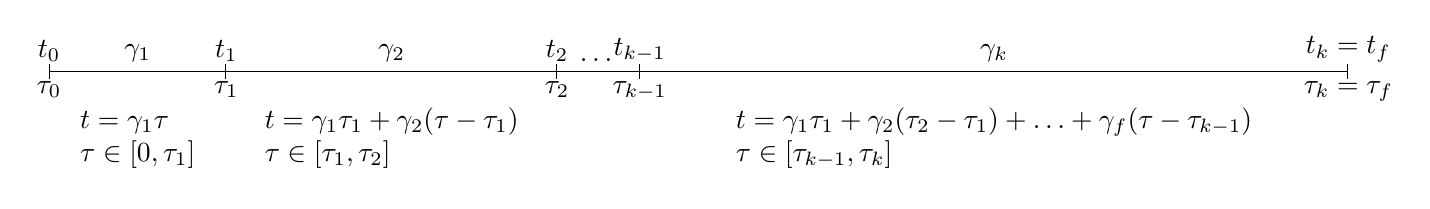
\begin{tikzpicture}[scale=1.5, domain=0:4, samples=200]
	    \draw [|-|](0,0) node[above] {$t_0$} node[below] {$\tau_0$} -- (1.5,0) node[midway, above] {$\gamma_1$} node[midway, below=0.3cm] {\begin{tabular}{l}
	    	$t = \gamma_1\tau$ \\
	    	$\tau\in[0, \tau_1]$
	    	\end{tabular}};
	    \draw [-|](1.5,0) node[above] {$t_1$} node[below] {$\tau_1$} -- (4.3,0) node[midway, above] {$\gamma_2$} node[midway, below=0.3cm] {\begin{tabular}{l}
	    	$t = \gamma_1\tau_1+\gamma_2(\tau-\tau_1)$ \\
	    	$\tau\in[\tau_1, \tau_2]$
	    	\end{tabular}};
	    \draw [-|](4.3,0) node[above] {$t_2$} node[below] {$\tau_2$} -- (5,0) node[midway,above] {\dots};
	    \draw [-|](5,0) node[above] {$t_{k-1}$} node[below] {$\tau_{k-1}$} -- (11,0) node[midway, above] {$\gamma_k$} node[midway, below=0.3cm] {\begin{tabular}{l}
	    	$t = \gamma_1\tau_1+\gamma_2(\tau_2-\tau_1)+\dots+\gamma_f(\tau-\tau_{k-1})$ \\
	    	$\tau\in[\tau_{k-1}, \tau_k]$
	    	\end{tabular}} node[above] {$t_k = t_f$} node[below] {$\tau_k = \tau_f$};
	\end{tikzpicture}
	\vspace{2mm}
	\caption{Mehrere miteinander gekoppelte Zeitintervalle, die sich zu einem Gesamtintervall $[\tau_0, \tau_f]$ zusammensetzen.}
	\label{fig:Zeittransformation}
\end{figure}
Für die einzelnen Teilintervalle gelten dabei die dargestellten Zeittransformationen, sodass für das $j$-te Teilintervall
\begin{equation}
	\dTtransoftau = \gamma_j \,, \quad\textrm{mit}\, j=1,2,...,k
\end{equation}
und damit 
\begin{equation}
\ve{z}_j'(\tau) = 
\gamma_j
\begin{bmatrix}
\ve{f}(\xoftau,\uoftau,\tau) \\
-\frac{\partial H}{\partial \ve{x}}
\end{bmatrix} 
\end{equation} 
gilt. Auch hier lassen sich die festen Intervallgrenzen ohne Einschränkung der Allgemeinheit zu
\begin{equation}
	\tau_0 = 0\,, \quad\tau_j = j\,, \quad\textrm{mit}\, j=1,2,...,k
\end{equation}
wählen, sodass für die freien Intervallgrenzen 
\begin{align}
t_0 &= \tau_0 = 0\\
t_1 &= \gamma_1 \\
t_2 &= \gamma_1+\gamma_2 \\ 
\nonumber &\vdots\\ 
t_f = t_k &= \gamma_1+\gamma_2+\dots+\gamma_k 
\end{align}
gilt. Mithilfe dieser Erweiterung lassen sich beliebig viele Intervalle fester Intervallgrenzen auf Intervalle freier Grenzen transformieren. Eine Anwendung derartig verknüpfter Zeittransformationen kann nützlich sein, wenn mehrere \gls{OP}, die jeweils für ein Teilintervall gelten, betrachtet werden und die Übergangsstellen $t_j$ frei und damit Teil der Optimierung sein sollen. Dann lassen sich die entsprechenden Teilintervalle mit festen Grenzen definieren und wie dargestellt mithilfe der Transformationsvorschriften auf die gesuchten, freien Intervallgrenzen abbilden.
\section{Variationsprobleme mit internen Gleichungsnebenbedingungen}\label{sec:InterneGNB}
Es kann durchaus von Interesse sein, neben den Randbedingungen an den Zeitpunkten $t_0$ und $t_f$ zusätzliche interne Randbedingungen der Form
\begin{equation}
	\tilde{\mathbf{g}}(\xoftone,t_1) = 0 \label{eq:NBt1}
\end{equation} zu formulieren, die die optimalen Trajektorien erfüllen sollen, wenn das dynamische System beispielsweise einen bestimmten Zustand zu einem gewissen Zeitpunkt $t_1$ erreichen soll \cite{Papageorgiou.2012}. Dazu wird auch in diesem Fall das Gütefunktional in Gleichung \eqref{eq:J_var_sys} analog zur Betrachtung allgemeiner Endbedingungen erweitert und lautet 
\begin{equation}
\begin{split}
J(\ve{x},\dx,\ve{u},t,t_f,t_1) &= \underbrace{\Vofxoftf + \ve{\nu}^T\mathbf{g}(\xoftf,t_f) + \Vofxoftone + \tilde{\ve{\nu}}^T\tilde{\mathbf{g}}(\xoftone,t_1)}_{\Vofxoftoftonefallgemein} \\
& \qquad +\int_{t_0}^{t_f}l(\ve{x},\ve{u},t) + \ve{\lambda}^T(\ve{f}(\ve{x},\ve{u},t) - \dx)~\dtint{t}\,. \label{eq:J_var_sys_t1}
\end{split}
\end{equation}
Allgemein können die Systemzustände und die adjungierten Zustände an der Stelle $t_1$ unstetig sein \cite{Gerdts.2010}, weshalb es zweckmäßig ist, die Zeitpunkte $t_1^-$ und $t_1^+$ als die Zeitpunkte unmittelbar vor und nach der Sprungstelle $t_1$ zu definieren. Der Zeitpunkt $t_1$ kann wie bereits der Endzeitpunkt $t_f$ entweder festgelegt oder frei sein. An der Übergangsstelle $t_1$ ergeben sich die Transversalitätsbedingungen \cite{Gerdts.2010}
\begin{align}
\Big(\frac{\partial \tilde{V}}{\partial \xoftone} + \Big(\frac{\partial \tilde{\mathbf{g}}}{\partial \xoftone}\Big)^T\tilde{\ve{\nu}} - \lambdaoftone\Big)\Big|_{t_1=t_1^-} &= 0 \label{eq:Sprungbedingung1}\\
\Big(\frac{\partial \tilde{V}}{\partial \xoftone} + \Big(\frac{\partial \tilde{\mathbf{g}}}{\partial \xoftone}\Big)^T\tilde{\ve{\nu}} + \lambdaoftone\Big)\Big|_{t_1=t_1^+} &= 0 \label{eq:Sprungbedingung2}\\
H(\ve{x},\ve{u},\ve{\lambda},t)\Big|_{t=t_1^-} - H(\ve{x},\ve{u},\ve{\lambda},t)\Big|_{t=t_1^+} + \Big(\frac{\partial \tilde{V}}{\partial t}+\Big(\frac{\partial \tilde{\mathbf{g}}}{\partial t}\Big)^T\tilde{\ve{\nu}}\Big)\Big|_{t=t_1}&= 0\,,\quad \textrm{falls, $t_1$ frei ist.}\label{eq:Transversalität_t1}
\end{align}
Zwei Spezialfälle spielen für die Anwendung der zusätzlichen Transveralitätsbedingungen eine besondere Rolle und sollen an dieser Stelle hervorgehoben werden: 
\begin{enumerate}
	\item Wie bereits erwähnt können die Systemzustände \xoft~an der Übergangsstelle $t_1$ allgemein unstetig sein und einen Sprung aufweisen. Bei der Behandlung dynamischer Systeme, die ein reales System repräsentieren, ist ein derartiges sprunghaftes Verhalten oftmals unerwünscht, da es einerseits nicht realisierbar ist und andererseits unkomfortable Trajektorien bedeutet. Daher sind häufig solche Lösungen von Interesse, bei denen zumindest die Systemzustände \xoft~in $t_1$ stetig sind, also 
	\begin{equation}
		\xoftoneminus = \xoftoneplus \label{eq:Stetigkeit_t1}
	\end{equation}
	gilt. Damit lassen sich die Randbedingungen \eqref{eq:Sprungbedingung1} und \eqref{eq:Sprungbedingung2} zur sogenannten \textit{ersten Weierstrass-Erdmannschen-Eckenbedingung} zusammenfassen \cite{Gerdts.2010}:
	\begin{equation}
		2\Big(\frac{\partial \tilde{V}}{\partial \xoftone} + (\frac{\partial \tilde{\mathbf{g}}}{\partial \xoftone})^T\tilde{\ve{\nu}}\Big) - \lambdaoftoneminus + \lambdaoftoneplus = 0\,. \label{eq:WeierstrassErdmann1}
	\end{equation}
	Die adjungierten Zustände \lambdaoft~können dabei in $t_1$ weiterhin sprunghaft sein, was allerdings nicht problematisch ist, da sie keine physikalischen Größen darstellen.
	\item Der zweite Sonderfall ergibt sich, wenn $t_1$ zwar frei ist, aber die Nebenbedingung \eqref{eq:NBt1} und die zusätzlichen Kosten \Vofxoftone~nicht explizit von $t_1$ abhängen, also $\tilde{\mathbf{g}}(\xoftone) = 0$ und $\tilde{V}(\ve{x}(t_1))$ gilt. Gleichung \eqref{eq:Transversalität_t1} wird dann zur \textit{zweiten Weierstrass-Erdmannschen-Eckenbedingung}, aus der die Stetigkeit der Hamilton-Funktion in $t_1$ folgt \cite{Gerdts.2010}:
	\begin{equation}
	H(\ve{x},\ve{u},\ve{\lambda},t)_{|t=t_1^-} = H(\ve{x},\ve{u},\ve{\lambda},t)_{|t=t_1^+}\,. \label{eq:WeierstrassErdmann2}
	\end{equation}
\end{enumerate}
\section{Diskontinuierliche Systemdynamik}\label{sec:Diskontinuität}
Die Verwendung von diskontinuierlicher Systemdynamik liefert eine überaus nützliche Methode zur Betrachtung abschnittsweise unterschiedlicher Zustandsgleichungen in einem \gls{OP}. Mithilfe dieser Methode können verschiedene, in unterschiedlichen Bereichen geltende Systembeschreibungen in einem \gls{OP} verwendet werden, sodass sich einzelne Szenarien miteinander zu einem Gesamtszenario kombinieren lassen. Diese Methode findet bspw. in dem in Abschnitt \ref{subsec:Optimalitätsprinzip} skizzierten Abbiegeszenario Verwendung. Die drei Teilszenarien Gerade, Kurve und Gerade lassen sich mithilfe von Übergangsbedingungen verknüpfen und in den einzelnen Teilbereichen gilt jeweils die für das entsprechende Teilszenario formulierte Systemdynamik. Die Übergangsbedingungen, die den Wechsel von einer Systemdynamik zur nächsten angeben, sind dabei über die vom Fahrzeug zurückgelegte Strecke definiert. Die Verwendung der Strecke als Übergangskriterium hat den Vorteil, dass die zu verwendende Systemdynamik immer eindeutig ist. Die von einem realen Fahrzeug zurückgelegte Strecke kann zu keinem zukünftigen Zeitpunkt geringer sein als zu einem vorherigen Zeitpunkt, weshalb die Strecke eine monoton steigende Größe ist. Daher werden die Bereiche der einzelnen Systemdynamiken immer in der selben Reihenfolge durchlaufen. Die Systemdynamik eines Gesamtszenarios, bei dem die Strecke als Übergangskriterium verwendet wird und die Übergange immer in einer festen Reihenfolge ablaufen, lässt sich allgemein aus $k$ Teilszenarien wie folgt zusammensetzen \cite{Papageorgiou.2012}:
\begin{equation}
\dx = \ve{F}(\ve{x},\ve{u},t) = \left\{\begin{matrix*}[l]
\ve{f}_1(\ve{x},\ve{u},t)\,, & \mathrm{falls} & \begin{matrix}\tilde{{g}}_i(\ve{x},t) < 0 &\forall\, i = 1,2,...,k-1\end{matrix}\\
&\\
\ve{f}_2(\ve{x},\ve{u},t)\,, & \mathrm{falls} & 
\begin{matrix*}[l]
\tilde{{g}}_{\hat{i}}(\ve{x},t) \geq 0 &\forall\, \hat{i} = 1 &\textrm{und} \\ \tilde{{g}}_i(\ve{x},t) < 0 &\forall\, i = 2,...,k-1&
\end{matrix*}
\\
\vdots & & \\
\ve{f}_j(\ve{x},\ve{u},t)\,, & \mathrm{falls} & \begin{matrix*}[l]
\tilde{{g}}_{\hat{i}}(\ve{x},t) \geq 0 &\forall \, \hat{i} = 1,2,...,j-1 &\textrm{und} \\ \tilde{{g}}_i(\ve{x},t) < 0 &\forall\, i = j,...,k-1&
\end{matrix*}\\
\vdots & & \\
\ve{f}_k(\ve{x},\ve{u},t)\,, & \mathrm{falls} & \begin{matrix}\tilde{{g}}_{\hat{i}}(\ve{x},t) \geq 0 &\forall\, \hat{i} = 1,2,...,k-1
\end{matrix}
\end{matrix*}\right. \label{eq:Diskontinuität}
\end{equation}
Die skalaren Gleichungen $\tilde{{g}}_i(\xofti,t_i) = 0$ nehmen dabei die Funktion der $k-1$ Übergangsbedingungen zu den Zeitpunkten $t_i$ ein, zu denen von der einen Systemdynamik zur nächsten gewechselt wird, und werden analog zu den Ausführungen in Abschnitt \ref{sec:InterneGNB} wie interne \gls{GNB} behandelt. Für jeden der Übergangspunkte gelten die Transversalitätsbedingungen \eqref{eq:Sprungbedingung1}--\eqref{eq:Transversalität_t1} bzw. \eqref{eq:Stetigkeit_t1}--\eqref{eq:WeierstrassErdmann2}, wobei insbesondere bei der zweiten Weierstrass-Erdmannschen-Eckenbedingung darauf geachtet werden muss, dass sich auch die Hamilton-Funktion aufgrund der wechselnden Systemdynamik gemäß
\begin{equation}
	H_j(\ve{x},\ve{u},\ve{\lambda},t) = l(\ve{x},\ve{u},t) + \ve{\lambda}^T\ve{f}_j(\ve{x},\ve{u},t) \label{eq:Hamilton_j}
\end{equation} 
verändert. Damit lautet die zweite Weierstrass-Erdmannsche-Eckenbedingung in Gleichung \eqref{eq:WeierstrassErdmann2} an der Übergangsstelle $t_i$
\begin{equation}
H_i(\ve{x},\ve{u},\ve{\lambda},t)_{|t=t_i^-} = H_{i+1}(\ve{x},\ve{u},\ve{\lambda},t)_{|t=t_i^+}\,. \label{eq:WeierstrassErdmann2_j}
\end{equation}

Die in diesem Kapitel beschriebenen Methoden liefern die notwendigen Mittel, um dynamische \gls{OP} mithilfe der Variationsrechnung zu lösen und die Problemstellung so zu formulieren, dass komplexe Fahrszenarien durch geschickte Kombination mehrerer Teilszenarien vereinfacht und analytisch gelöst werden können. Das Optimalitätsprinzip nach Bellmann (siehe Abschnitt \ref{subsec:Optimalitätsprinzip}) liefert die Grundlage dafür, dass sich mehrere Teilprobleme zur optimalen Lösung eines Gesamtproblems zusammensetzen lassen. Mithilfe von Zeittransformationen und unter Verwendung diskontinuierlicher Systemdynamik (Abschnitte \ref{sec:Zeittransformation} und \ref{sec:Diskontinuität}) lassen sich auf frei wählbaren Zeitintervallen beliebig viele Teilsysteme unterschiedlicher Systemdynamik miteinander kombinieren, wobei sich mithilfe der Nebenbedingungen an den internen Übergangspunkten (siehe Abschnitt \ref{sec:InterneGNB}) Stetigkeit der Systemzustände erzielen lässt, während weiterhin die Optimalität der Lösung gewährleistet ist.
\section{Numerische Lösungsverfahren}\label{sec:Lösungsverfahren}
Dieser Abschnitt dient der Übersicht über unterschiedliche numerische Lösungsverfahren für dynamische \gls{OP}. Dazu sollen einige Verfahren erläutert und hinsichtlich ihrer Vor- und Nachteile miteinander verglichen werden. Zunächst wird der Unterschied zwischen \textit{indirekten} und \textit{direkten} Lösungsverfahren erklärt und anschließend jeweils verschiedene Verfahren der beiden Verfahrensklassen vorgestellt.
\subsection{Indirekte Lösungsverfahren}\label{subsec:Indirekt}
Bei den indirekten Lösungsverfahren wird mithilfe der Optimalitätsbedingungen \eqref{eq:Zustandsdgl}--\eqref{eq:Steuerungsgleichung} und der Randbedingungen \eqref{eq:Anfangswerte}--\eqref{eq:Transversalitaet} das entstehende Randwertproblem gelöst \cite{Papageorgiou.2012} -- die indirekten Lösungsverfahren basieren also auf der Anwendung der Variationsrechnung. Die Lösung kann dabei entweder analytisch oder mithilfe numerischer Verfahren ermittelt werden \cite{Gerdts.2010}. Bei indirekten Verfahren wird das dynamische \gls{OP} nicht zunächst diskretisiert, sondern es werden direkt die Optimalitätsbedingungen für das entsprechende \gls{OP} hergeleitet, weshalb bei den indirekten Verfahren auch von einer \glqq\textit{first-optimize-then-discretize\grqq}-Strategie gesprochen wird \cite{Papageorgiou.2012} -- dies trifft insbesondere auf indirekte Diskretisierungsverfahren zu (siehe Abschnitt \ref{subsubsec:Diskretisierungsverfahren_indirekt}). Dadurch, dass das dynamische \gls{OP} bei indirekten Verfahren nicht zuerst in ein statisches Ersatzproblem umgewandelt, sondern stattdessen mithilfe der Variationsrechnung ein Randwertproblem gelöst wird, besitzen sie den großen Vorteil, dass sie zum einen Informationen über die Struktur der optimalen Lösung liefern und sich zum anderen eine sehr hohe Lösungsgenauigkeit erzielen lässt \cite{KnutGraichen.2012}. Selbst wenn das Randwertproblem nicht analytisch gelöst werden kann, so lassen sich trotzdem aus der Lösung der kanonischen \gls{DGL} Erkenntnisse gewinnen, die vor allem für die Interpretation der optimalen Trajektorien sehr wertvoll sein können. Ein weiterer Vorteil indirekter Lösungsverfahren ist, dass die adjungierten Zustände zur Sensitivitätsanalyse des Gütefunktionals gegenüber Änderungen der Anfangszustände \xzero~verwendet werden können \cite{KnutGraichen.2012}. Indirekte Lösungsverfahren haben den Nachteil, dass die Lösbarkeit eines dynamischen \gls{OP} -- also die Herleitung der kanonischen \gls{DGL} und das daraus resultierende Randwertproblem -- von der Struktur des \gls{OP} selbst abhängt. Die Optimalitätsbedingungen und die Randbedingungen aufzustellen kann für komplizierte Systeme sehr aufwendig sein \cite{Papageorgiou.2012}. Außerdem benötigen indirekte Lösungsverfahren häufig Startschätzungen für die adjungierten Zustände. Die Schätzung dieser Initialwerte beeinflusst die Qualität der Lösung bzw. ob das Verfahren überhaupt konvergiert, sodass der Konvergenzbereich indirekter Verfahren oftmals nicht sehr groß ist \cite{Papageorgiou.2012}. Nachfolgend werden einige indirekte Lösungsverfahren vorgestellt und hinsichtlich des \gls{AD}-Planungsproblems diskutiert. 
\subsubsection{Indirekte Diskretisierungsverfahren}\label{subsubsec:Diskretisierungsverfahren_indirekt}
Das \glqq first-optimize-then-discretize\grqq-Paradigma trifft vor allem auf indirekte Diskretisierungverfahren zu. Wie bei allen indirekten Lösungsverfahren werden entsprechend der Ausführungen in Abschnitt \ref{sec:dynamischeOpt} die \gls{DGL} \eqref{eq:Sysdyn_z} über den Ansatz der Variationsrechnung hergeleitet. Gemeinsam mit den Randbedingungen \eqref{eq:Anfangswerte}--\eqref{eq:Transversalitaet} ergibt sich ein \gls{ZPR}, welches auf dem Gesamtintervall $[t_0, t_f]$ an $N+1$ Stützstellen diskretisiert wird \cite{KnutGraichen.2012} -- das Problem wird also zuerst optimiert und anschließend diskretisiert. Dieses Randwertproblem wird unter Berücksichtigung der Randbedingungen mithilfe eines numerischen Integrationsverfahrens gelöst, wie zum Beispiel dem Verfahren von Heun, bei dem ein Trapez zur Approximation des Integrals verwendet wird \cite{KnutGraichen.2012} (siehe auch \cite{Adamy.2009} für Informationen zu weiteren Verfahren). Da die zu lösenden \gls{DGL} bei der numerischen Integration durch Differenzenquotienten ersetzt werden, werden Diskretisierungsverfahren auch als Differenzenverfahren bezeichnet \cite{Ascher.1995c5}.
\begin{multicols}{2}
Vorteile:
	\begin{itemize}
		\item Numerische Robustheit aufgrund simultaner Berücksichtigung der kanonischen \gls{DGL} und Randbedingungen \cite{KnutGraichen.2012}.
		\item Erhöhung der Genauigkeit durch Steigerung der Anzahl der Diskretisierungsstellen \cite{KnutGraichen.2012}.
		\item Durch Anwendung von \gls{RKV} mit höherer Verfahrensordnung lässt sich die Genauigkeit der Integralapproximation verbessern \cite{Ascher.1995c5}.
	\end{itemize}
	
	\columnbreak
	
Nachteile:
	\begin{itemize}
		\item Steuergröße $\ve{u}$ muss explizit nach $\ve{x}$ und $\ve{\lambda}$ auflösbar sein \cite{KnutGraichen.2012}.\vspace{\fill}
		\item Gute Initialschätzung für \lambdaoftzero~notwendig \cite{KnutGraichen.2012}.\vspace{\fill}
		\item Größere Anzahl an Diskretisierungsstellen steigert den Rechenaufwand \cite{KnutGraichen.2012}.\vspace{\fill}
	\end{itemize}
\end{multicols}

\subsubsection{Indirekte Schießverfahren}\label{subsubsec:Schießverfahren_indirekt}
Im Gegensatz zu den indirekten Diskretisierungsverfahren wird beim Einfachschießverfahren die Lösung ausgehend von einem Anfangswertproblem berechnet \cite{Papageorgiou.2012}, anstatt ausgehend vom \gls{ZPR}. Dazu wird aus den Anfangswerten \xzero~und einer Initialschätzung $\ve{\lambda}_0^{(0)}$ für die adjungierten Zustände der Startvektor $\ve{z}_0 = \begin{bmatrix}\xzero^T & \ve{\lambda}_0^{(0)T}\end{bmatrix}^T$ gebildet. Von diesem Startvektor ausgehend werden die \gls{DGL} anschließend bis $t_f$ numerisch vorwärts integriert. Nach Abschluss der Integration erhält man ein Ergebnis für $\lambdaoftf^{(0)}$, welches mit den Randbedingungen \eqref{eq:Lambdaend} verglichen wird. Die Abweichungen in den Randbedingungen lassen sich durch den Fehlervektor $\ve{e}^{(l)} = \lambdaoftf - \ve{\lambda}(t_f)^{(l)}$ ausdrücken, der durch Verbesserung der Startschätzung $\ve{\lambda}_0^{(l)}$ so lange verringert wird, bis eine gewünschte Fehlertoleranz nicht mehr überschritten wird und damit das Ergebnis einer vorgegebenen Güte entspricht \cite{Papageorgiou.2012}. Der hochgestellte Index $(l)$ gibt dabei die $l$-te Iteration der Integration an. Der Startwert $\ve{\lambda}_0^{(l+1)}$ der nächsten Iteration kann zum Beispiel durch Anwendung des Newton-Verfahrens aktualisiert werden \cite{Papageorgiou.2012}.
Auch freie Endzeiten $t_f$ können bei den Schießverfahren berücksichtigt werden. Dazu wird analog zu den adjungierten Anfangszuständen eine Initialschätzung $t_f^{0}$ vorgegeben und der Fehlervektor um die Transversalitätsbedingung für freie Endzeit \eqref{eq:Transversalitaet} erweitert \cite{Papageorgiou.2012}.
\newpage
\begin{multicols}{2}
	Vorteile:
	\begin{itemize}
		\item \glqq Einfache\grqq Methode mit geringem Implementierungsaufwand \cite{Ascher.1995c4}.
		\item Mehrfachschießverfahren bieten die Möglichkeit der Parallelisierung \cite{Betts.1998}.\vspace{\fill}
		\item[\vspace{\fill}]
	\end{itemize}
	
	\columnbreak
	
	Nachteile:
	\begin{itemize}
		\item Die Steuergröße $\ve{u}$ muss explizit nach $\ve{x}$ und $\ve{\lambda}$ auflösbar sein \cite{Papageorgiou.2012}.\vspace{\fill}
		\item Instabile Anfangswertprobleme führen dazu, dass das Einfachschießverfahren instabil wird \cite{Ascher.1995c4}, wobei gezeigt werden kann, dass die kanonischen \gls{DGL} im linearen Fall immer an der imaginär Achse gespiegelte Eigenwerte und damit instabile Eigenmoden besitzen, selbst wenn das lineare System stabil ist \cite{KnutGraichen.2012}. 
		\item Empfindlichkeit gegenüber schlechten Startschätzungen für $\ve{\lambda}_0^{(0)}$, sodass unter Umständen keine Lösung auf dem gesamten Integrationsintervall $[t_0, t_f]$ gefunden werden kann \cite{Ascher.1995c4}.
		\item Eingeschränkte Anwendbarkeit aufgrund der numerischen Berechnungsschwierigkeiten -- vor allem für kleine Probleme mit wenigen Zuständen geeignet \cite{Papageorgiou.2012}.
	\end{itemize}
\end{multicols}

Dem Problem der numerischen Stabilität und dem Umstand, dass das Anfangswertproblem ggf. nicht bis zur rechten Intervallgrenze integriert werden kann, kann mit dem Mehrfachschießverfahren begegnet werden. Ähnlich zu den Diskretisierungsverfahren wird das Integrationsintervall beim Mehrfachschießverfahren ebenfalls in $N$ Subintervalle aufgeteilt. Auf jedem der Subintervalle wird das Anfangswertproblem \eqref{eq:Sysdyn_z} mit $\ve{z}(t_j) = \begin{bmatrix}\ve{x}_j^T & \ve{\lambda}_j^T\end{bmatrix}^T$ und $t\in[t_j, t_{j+1}),\,j = 0,1,...,N-1$ mittels Einfachschießverfahren gelöst \cite{Gerdts.2010}. Damit die Lösung der einzelnen Anfangswertprobleme auf den Subintervallen tatsächlich eine Lösung des ursprünglichen \gls{ZPR} ist, müssen neben den Randbedingungen, die sich über die Formulierung der Optimalitätsbedingungen ergeben, zusätzlich noch die Stetigkeitsbedingungen 
\begin{equation}
	\begin{bmatrix}
	\ve{z}_0(t_1,\begin{bmatrix}\ve{x}_0^T & \ve{\lambda}_0^T\end{bmatrix}^T) - \begin{bmatrix}\ve{x}_1^T & \ve{\lambda}_1^T\end{bmatrix}^T \\
	\ve{z}_1(t_2,\begin{bmatrix}\ve{x}_1^T & \ve{\lambda}_1^T\end{bmatrix}^T) - \begin{bmatrix}\ve{x}_2^T & \ve{\lambda}_2^T\end{bmatrix}^T \\
	\vdots \\
	\ve{z}_{N-2}(t_{N-1},\begin{bmatrix}\ve{x}_{N-2}^T & \ve{\lambda}_{N-2}^T\end{bmatrix}^T) - \begin{bmatrix}\ve{x}_{N-1}^T & \ve{\lambda}_{N-1}^T\end{bmatrix}^T
	\end{bmatrix} = \ve{0}
\end{equation}
zwischen den einzelnen Subintervallen erfüllt sein \cite{Gerdts.2010}. Das Ergebnis des Anfangswertproblems am Intervallende des $j$-ten Subintervalls muss also dem Anfangswert der Lösung auf dem $j+1$-ten Intervall entsprechen. Mit dieser Erweiterung auf das Mehrfachschießverfahren lässt sich die Robustheit der numerischen Integration auf Kosten des Rechenaufwands steigern, da der Rechenaufwand durch die Intervallunterteilung ansteigt \cite{Betts.1998}.
\subsubsection{Indirekte Gradientenverfahren}\label{subsubsec:Gradientenverfahren_indirekt}
Indirekte Gradientenverfahren werden überwiegend für Probleme mit fester Endzeit $t_f$ und freien Endzuständen \xoftf~verwendet \cite{KnutGraichen.2012}. Aus den freien Endzuständen folgt mit Gleichung \eqref{eq:Lambdaend} die Festlegung von Endwerten für die adjungierten Zustände, während die Anfangszustände \xzero~über Gleichung \eqref{eq:Anfangswerte} vorgegeben sind. Dadurch ergeben sich $n$ Anfangsbedingungen für die Systemzustände und $n$ Endbedingungen für die adjungierten Zustände. Bei einer derartigen Vorgabe von Randwerten (festes \xoftzero, festes \lambdaoftf) wird auch von entkoppelten Randbedingungen gesprochen, da man an den beiden Randpunkten $t_0$ und $t_f$ jeweils nur Randbedingungen entweder für die Systemzustände $\ve{x}$ oder für die adjungierten Zustände $\ve{\lambda}$ erhält\footnote{Die hier ausgenutzte Eigenschaft entkoppelter Randbedingungen ist nicht zu verwechseln mit separierten Randbedingungen (siehe Abschnitt \ref{sec:dynamischeOpt}).} \cite{KnutGraichen.2012}. Diese Eigenschaft machen sich die Gradientenverfahren zu nutze, da das Optimalsteuerungsproblem sequenziell durch abwechselnde Vorwärts- und Rückwärtsintegration ausgehend von den gegebenen Randwerten \xoftzero~bzw. \lambdaoftf~gelöst wird \cite{KnutGraichen.2012}. Wird nun eine Steuertrajektorie $\ve{u}$ durch Initialisierung als gegeben angenommen, dann lassen sich die Systemgleichungen \eqref{eq:Zustandsdgl} ausgehend von \xzero~durch Vorwärtsintegration von $t_0$ bis $t_f$ lösen. Analog dazu lassen sich die \gls{DGL} der adjungierten Zustände \eqref{eq:Adjdgl} ausgehend von \lambdaoftf~durch Rückwärtsintegration von $t_f$ bis $t_0$ bestimmen. Dadurch hängt der Wert des Gütefunktionals nur noch von $\ve{u}$ ab \cite{Papageorgiou.2012}. Aus dieser Eigenschaft lässt sich der Gradient des Gütefunktionals bezüglich der Steuertrajektorie als
\begin{equation}
	\frac{\partial J}{\partial \ve{u}} = \int_{t_0}^{t_f}\frac{\partial l(\ve{x},\ve{u},t) + \ve{\lambda}^T\ve{f}(\ve{x},\ve{u},t)~\dtint{t}}{\partial \ve{u}} = \int_{t_0}^{t_f}\frac{\partial H(\ve{x},\ve{u},\ve{\lambda},t)~\dtint{t}}{\partial \ve{u}}
\end{equation}
bestimmen, der angibt, wie sich der Wert des Gütefunktionals bei Änderungen der Steuertrajektorie verhält \cite{Papageorgiou.2012}. Da die Eingangstrajektorie $\ve{u}$ während des Gradientenverfahrens iterativ verbessert wird und dadurch der optimalen Lösung $\ve{u}^*$ mit jeder Iteration näher kommt, wird die Steuerungsgleichung \eqref{eq:Steuerungsgleichung} im Allgemeinen nicht erfüllt sein, sodass dieser Gradient ungleich null wird \cite{KnutGraichen.2012}. Gilt für den Gradienten $\frac{\partial J}{\partial \ve{u}} = 0$, so ist offensichtlich auch die Optimalitätsbedingung \eqref{eq:Steuerungsgleichung} erfüllt und $\ve{u}$ entspricht der optimalen Lösung $\ve{u}^*$. Dieser Gradient kann genutzt werden, um mithilfe einer Schrittweite $\alpha^{(l)}$ die Steuertrajektorie entsprechend der Richtung des Gradienten anzupassen, sodass  
\begin{equation}
\uoft^{(l+1)} = \uoft^{(l)} - \alpha^{(l)}(\frac{\partial J}{\partial \ve{u}})^{(l)}
\end{equation}
gilt \cite{KnutGraichen.2012}. Die Schrittweite $\alpha^{(l)}$ kann entweder fest sein oder über ein Liniensuchverfahren bestimmt werden \cite{Papageorgiou.2012}. Der hochgestellte Index $l$ gibt auch hier die Iteration des Algorithmus an. Mithilfe der aktualisierten Steuertrajektorie $\ve{u}^{(l+1)}$ kann wieder von vorne verfahren werden und es können erneut die Lösungen für $\ve{x}$ und $\ve{\lambda}$ durch Vorwärts- bzw. Rückwärtsintegration mit der neuen Steuertrajektorie berechnet werden \cite{Papageorgiou.2012}. Dieses Vorgehen wird so lange wiederholt, bis der Gradient klein genug ist und ein entsprechendes Abbruchkriterium erfüllt ist. Dann ist $\ve{u}$ nah genug an der optimalen Lösung \cite{Papageorgiou.2012}. Wie bereits bei den Schießverfahren gilt auch hier, dass die kanonischen \gls{DGL} im linearen Fall instabile Eigenmoden besitzen. Diese können prinzipiell sowohl in den Systemzuständen als auch in den adjungierten Zuständen auftreten. Da für die adjungierten Zustände allerdings keine Anfangswerte vorgegeben werden können und diese bei den meisten Lösungsverfahren bei der Initialisierung geschätzt werden müssen, sind diese für die Vorwärtsintegration aus numerischer Sicht kritischer. Da die Lösung der adjungierten Zustände bei den Gradientenverfahren allerdings in Rückwärtsrichtung geschieht (idealerweise ausgehend von festen Endwerten \lambdaoftf), entfällt bei den Gradientenverfahren die Startschätzung der adjungierten Zustände, sodass sie numerisch robust sind \cite{KnutGraichen.2012}.
\newpage
\begin{multicols}{2}
	Vorteile:
	\begin{itemize}
		\item Dadurch, dass der Gradient $\frac{\partial H}{\partial \ve{u}}$ explizit für das Auffinden der optimalen Steuertrajektorie verwendet wird, bieten sich Gradientenverfahren für Systeme an, bei denen sich $\ve{u}$ nicht explizit durch $\ve{x}$ und $\ve{\lambda}$ ausdrücken lässt \cite{KnutGraichen.2012}.
		\item Effiziente Lösung für Problemstellungen mit fester Endzeit und entkoppelten Randbedingungen \cite{Papageorgiou.2012}.
		\item Stellgrößenbeschränkungen können bei der Suche nach der zulässigen Richtung im Algorithmus berücksichtigt werden \cite{Papageorgiou.2012}.
		\item Numerisch robuste Lösung, da die adjungierten \gls{DGL} anstelle der numerisch instabilen Vorwärtsrichtung in Rückwärtsrichtung integriert werden und keine Startschätzung der adjungierten Zustände notwendig ist \cite{KnutGraichen.2012}.
	\end{itemize}
	
	\columnbreak
	
	Nachteile:
	\begin{itemize}
				\item Berücksichtigung zusätzlicher Beschränkungen bereitet konzeptuelle Schwierigkeiten \cite{Papageorgiou.2012}.\vspace{\fill}
				\item Erweiterung auf allgemeine Randbedingungen und freie Endzeit zwar möglich, allerdings auf Kosten schlechterer Kovergenzeigenschaften und Robustheit \cite{KnutGraichen.2012}.\vspace{\fill}
				\item Oftmals langsames Konvergenzverhalten in der Nähe des Optimums \cite{KnutGraichen.2012}.\vspace{\fill}
			    \item[\vspace{\fill}]
	\end{itemize}
\end{multicols}
\subsubsection{Indirekte Kollokationsverfahren}\label{subsubsec:Kollokationsverfahren_indirekt}
Zuletzt werden hier die indirekten Kollokationsverfahren erklärt. Wie bereits bei den indirekten Diskretisierungsverfahren wird auch bei den Kollokationsverfahren das Gesamtintervall $[t_0, t_f]$ zunächst in $N$ äquidistante Subintervalle unterteilt. Der Ansatz der Kollokationsverfahren besteht nun darin, dass die Lösung auf jedem der $N$ Subintervalle $[t_i, t_{i+1}],\, i = 0,1,...,N-1$ durch stückweise definierte Polynome $\ve{S}_i(t)$ approximiert wird \cite{Gerdts.2010} -- dies gilt sowohl für die Systemzustände als auch für die adjungierten Zustände. Dazu werden zusätzlich zu den Randpunkten der Subintervalle sogenannte Kollokationsstellen $t_{ij} \in [t_i, t_{i+1}],\, j = 1,...,k$ definiert, an denen durch die Kollokationsbedingungen  
\begin{equation}
	\dot{\ve{S}}_i(t_{ij}) = \ve{f}(t_{ij},\ve{S}_i(t_{ij})) \label{eq:Kollokationsbedingung}
\end{equation}
ein Übereinstimmen der Approximation und der kanonischen \gls{DGL} erzwungen wird \cite{Gerdts.2010}. Damit an den Intervallübergängen Stetigkeit gewährleistet ist, müssen die Approximationspolynome die Stetigkeitsbedingungen \eqref{eq:Stetigkeitsbedingung} zwischen zwei Subintervallen erfüllen. Dazu werden die zwei benachbarten Intervalle $[t_{i-1}, t_i]$ und $[t_i, t_{i+1}]$, die in einem beliebigen Punkt $t_i$ mit $0 < i < N-1$ ineinander übergehen, mit den dazugehörigen Polynomen $\ve{S}_{i-1}(t)$ und $\ve{S}_i(t)$ betrachtet. Diese müssen die Bedingung
\begin{equation}
\ve{S}_{i-1}(t_i) = \ve{S}_i(t_i) \label{eq:Stetigkeitsbedingung}
\end{equation} 
erfüllen. Zusätzlich müssen auch die Randbedingungen \eqref{eq:Anfangswerte}--\eqref{eq:Lambdaend} durch die Polynome erfüllt sein \cite{Gerdts.2010}. Es existieren verschiedene Möglichkeiten zur Wahl der Kollokationspunkte innerhalb eines Subintervalls (Lobatto-, Radau-, Gauss-Kollokation \cite{Weiss.1974}), wobei die Lobatto-Kollokation die effizienteste Wahl darstellt \cite{Weiss.1974}. Dafür werden insgesamt $k=3$ Kollokationspunkte gewählt: der Intervallanfang, die Intervallmitte und das Intervallende, womit 
\begin{equation}
	t_{ij} = t_{i+\frac{j-1}{2}}\,,\quad i = 0,1,...,N-1,\quad j = 1,...,k
\end{equation}
gilt \cite{Papageorgiou.2012}. Unter der Annahme, dass die Endzeit $t_f$ fest sei, ergibt sich ein $N\cdot (k+1)\cdot 2n$-dimensionales nichtlineares Gleichungssystem, welches aus den $N\cdot k\cdot 2n$ Kollokationsbedingungen \eqref{eq:Kollokationsbedingung}, den $(N-1)\cdot 2n$ Stetigkeitsbedingungen \eqref{eq:Stetigkeitsbedingung} der Approximationspolynome an den Intervallgrenzen $t_i$ und den $2n$ Randbedingungen \eqref{eq:Anfangswerte}--\eqref{eq:Lambdaend} besteht \cite{Gerdts.2010}. Mithilfe dieses Gleichungssystems lassen sich die unbekannten Polynomkoeffizienten bestimmen \cite{Gerdts.2010}. Für $N$ Intervalle mit je $2n$ Gleichungen dürfen pro Polynom maximal $k+1$ Koeffizienten auftreten damit das Gleichungssystem eindeutig lösbar ist. Unter Berücksichtigung der allgemeinen Struktur eines Polynoms von Grad $\rho$
\begin{equation}
	P(x) = a_{\rho+1}x^\rho + a_{\rho}x^{\rho-1} + ... + a_{1}x + a_0\,,
\end{equation}
lässt sich feststellen, dass dabei $\rho+1$ Koeffizienten auftreten. In \cite{Ascher.1995c5} konnte gezeigt werden, dass sich Kollokationsverfahren mit stückweise definierten Polynomen zur Lösung von \gls{ZPR} durch ein äquivalentes implizites \gls{RKV} ausdrücken lassen. Dabei gilt, dass bei Verwendung von $k$ Kollokationsstellen Polynome von (höchstens) Grad $k$ auftreten und sich ein äquivalentes $k$-stufiges \gls{RKV} ergibt \cite{Ascher.1995c5}. Die Berücksichtigung freier Endzeiten bei Kollokationsverfahren lässt sich wie in \ref{sec:Zeittransformation} beschrieben umsetzen. 
\begin{multicols}{2}
	Vorteile:
	\begin{itemize}
		\item Effektiv anwendbar zur Lösung von \gls{MPR}, die speziell bei der Optimierung von Trajektorien auftauchen \cite{Betts.1998}.
		\item Vergleichsweise geringer Rechenaufwand, insbesondere wenn die Randbedingungen separiert sind (siehe Abschnitt \ref{sec:dynamischeOpt}) \cite{Cash.1980}.
		\item Es lassen sich Ergebnisse mit hoher Genauigkeit erzielen bei überschaubarem Rechenaufwand \cite{Cash.1980}.
	\end{itemize}
	
	\columnbreak
	
	Nachteile:
	\begin{itemize}
		\item Übereinstimmung der \gls{DGL} mit der Approximation nur an den Kollokationsstellen \cite{Betts.1998}.	
		\item Wie bei allen indirekten Lösungsverfahren müssen die Optimalitätsbedingungen \eqref{eq:Zustandsdgl}--\eqref{eq:Steuerungsgleichung} und die dazugehörigen Randbedingungen \eqref{eq:Anfangswerte}--\eqref{eq:Transversalitaet} hergeleitet werden \cite{Betts.1998}.

		\item[\vspace{\fill}]
	\end{itemize}
\end{multicols}
\subsection{Direkte Lösungsverfahren}\label{subsec:Direkt}
Unabhängig davon, wie genau ein allgemeines dynamisches \gls{OP} (\eqref{eq:J_dyn}--\eqref{eq:UNB}) durch ein bestimmtes direktes Lösungsverfahren gelöst wird, haben alle direkten Verfahren eines gemeinsam: Das dynamische \gls{OP} wird mittels Diskretisierung in ein statisches Ersatzproblem überführt, wobei die Steuertrajektorie \uoft~an $N$ Stützstellen diskretisiert wird \cite{KnutGraichen.2012}. Dadurch wird aus dem dynamischen \gls{OP} ein endlich dimensionales statisches \gls{OP}, welches in der allgemeinen Form \eqref{eq:J_statisch}--\eqref{eq:UNB_statisch} geschrieben werden kann und bezüglich der Optimierungsvariablen $\ve{u}_i$ mit $i=0,1,...N-1$ optimiert wird. Ein wesentlicher Unterschied zwischen direkten und indirekten Verfahren liegt darin, dass die Optimalitätsbedingungen aus der Variationsrechnung bei direkten Verfahren nicht explizit berücksichtigt werden müssen \cite{Rathgeber.2016}. Diese Eigenschaft macht direkte Lösungsverfahren besonders attraktiv für komplizierte Anwendungen \cite{Betts.1998}. Aufgrund dieser Vorgehensweise werden direkte Verfahren auch als \glqq\textit{first-discretize-then-optimize\grqq}-Strategie bezeichnet \cite{Papageorgiou.2012}. Ungeachtet der Komplexität der Lösung lässt sich das dynamische \gls{OP} mithilfe der Diskretisierung immer auf ein statisches Ersatzproblem zurückführen, wodurch sich direkte Methoden robust anwenden lassen und sich vielseitige Anwendungsbereiche ergeben \cite{Betts.1998}. Weitere Vorteile direkter Lösungsverfahren liegen zum einen darin, dass sich aufgrund der Diskretisierung der Trajektorien Zustandsbeschränkungen sowohl in Form von \gls{GNB} als auch \gls{UNB} leicht berücksichtigen lassen \cite{KnutGraichen.2012}. Zum anderen hängt die Qualität der Lösung nicht von Startschätzungen für die adjungierten Zustände ab, die bei indirekten Verfahren angegeben werden müssen, weshalb sich oftmals größere Konvergenzbereiche für direkte Verfahren ergeben \cite{KnutGraichen.2012}. Ein Nachteil von direkten Lösungsverfahren liegt darin, dass die Optimierungsvariablen das optimale Systemverhalten nur an den diskretisierten Stützstellen wiedergeben, weshalb direkte Verfahren ggf. nicht die gewünschte Lösungsgenauigkeit erreichen \cite{Papageorgiou.2012}. Außerdem liefert die Lösung keine Erkenntnisse über die analytische Struktur der optimalen Verläufe. Mithilfe einer höherfrequenten Diskretisierung in engeren Schritten lässt sich die Übereinstimmung der direkten Lösung mit dem analytischen Verlauf der optimalen Lösung und damit die Qualität der direkten Lösung verbessern, allerdings bedeutet dies eine Zunahme der Dimension des Problems. Gerade Systeme hoher Ordnung können auf diese Weise schnell in eine Größenordnung anwachsen, sodass sie sich nicht mehr oder nur sehr langsam lösen lassen, abhängig davon, wie viel Rechenleistung und Speicherkapazität zur Verfügung stehen \cite{Papageorgiou.2012}. Dies war lange Zeit ein maßgeblich beschränkender Faktor in der Anwendung direkter Lösungsverfahren, der mittlerweile aufgrund des heutigen Fortschritts bei der Entwicklung leistungsfähiger Rechner immer mehr in den Hintergrund gerückt ist \cite{Papageorgiou.2012}. 

Für die Klasse der direkten Lösungsverfahren lässt sich zu jedem vorgestellten indirekten Verfahren ein direktes Lösungsverfahren angeben, welches sehr eng mit der indirekten Lösungsvariante verwandt ist (direkte Voll-/Teildiskretisierungsverfahren, direkte Einfach-/Mehrfachschießverfahren, direkte Kollokationsverfahren, direkte Gradientenverfahren). Das Ziel dieser Arbeit besteht jedoch darin, den großen Vorteil indirekter Lösungsverfahren auszunutzen und durch den Lösungsweg über die Variationsrechnung Informationen über die Struktur der optimalen Trajektorien zu erhalten. Aus diesem Grund werden die direkten Lösungsverfahren nicht weiter vertieft und es sei an dieser Stelle auf entsprechende Fachliteratur verwiesen \cite{KnutGraichen.2012,Gerdts.2010,Papageorgiou.2012,Ascher.1995c4,Ascher.1995c5,Betts.1998,Cervantes.2009}.
\subsection{Diskussion der Lösungsverfahren}\label{subsec:Diskussion}
Nachdem nun einige Lösungsverfahren vorgestellt und der Unterschied zwischen indirekten und direkten Verfahren zur numerischen Lösung von Randwertproblemen dargelegt wurde, sollen die Ergebnisse der vorangegangenen Abschnitte diskutiert und in den Kontext des \gls{AD}-Planungsproblems eingeordnet werden -- die direkten Lösungsverfahren werden dabei aus den o.g. Gründen nicht weiter berücksichtigt. 

Jedes der beschriebenen indirekten Lösungsverfahren hat seine Vor- und Nachteile und ist daher für gewisse Systemklassen mehr oder weniger geeignet. Wie in Kapitel \ref{cha:Modellbildung} beschrieben ergeben sich für das \gls{AD}-Planungsproblem je nach Fahrszenario und Detaillierungsgrad Systeme unterschiedlicher Ordnung. Wird die Stellgröße des Systems quadratisch bestraft, sodass das Gütefunktional immer einen energieoptimalen Anteil enthält \cite{KnutGraichen.2012}, lässt sich die Stellgröße immer in Abhängigkeit von $\ve{x}$ und $\ve{\lambda}$ ausdrücken, sodass dieser Nachteil bei allen indirekten Verfahren zu vernachlässigen ist. Der in Abschnitt \ref{subsubsec:Singularität} beschriebene singuläre Fall tritt bei dieser Art von Gütefunktionalen nicht auf. In allen betrachteten Szenarien besitzt das Gesamtsystem bestehend aus den Systemzuständen und den adjungierten Zuständen immer an der Imaginärachse gespiegelte Eigenwerte und ist damit instabil, weshalb eine Vorwärtsintegration der adjungierten Zustände problematisch ist -- insbesondere deshalb, weil eine gute Startschätzung der adjungierten Zustände ohne vorherige Kenntnis der Lösungstrajektorien nicht möglich ist. Aus diesem Grund ist das indirekte Einfachschießverfahren nicht für die Lösung komplizierterer Systeme geeignet. Zwar lässt sich die numerische Stabilität mithilfe des Mehrfachschießverfahrens verbessern, allerdings steigt dadurch der Rechenaufwand, weshalb auch dieses Verfahren als ungeeignet bewertet wird. 

Das indirekte Diskretisierungsverfahren ist gegenüber den Schießverfahren numerisch deutlich robuster, da anstelle eines Anfangswertproblems ein Randwertproblem gelöst wird und dadurch die kompletten Randbedingungen immer berücksichtigt werden. Allerdings muss die Diskretisierungsschrittweite für eine genaue Lösung möglichst klein gewählt werden, wodurch der Rechenaufwand stark ansteigt. Dies zeigt sich vor allem dann, wenn die optimalen Trajektorien für ein großes Zeitintervall bestimmt werden sollen. Werden beispielsweise die kanonischen \gls{DGL} für ein dreistufiges Integratorsystem hergeleitet, ergibt sich ein Gesamtsystem 6. Ordnung. Soll für dieses System das Randwertproblem mithilfe des indirekten Diskretisierungsverfahrens mit einer Schrittweite von $T_s = 0.1\unit{s}$ gelöst werden, steigt die Anzahl der Optimierungsvariablen um 60 zusätzliche Variablen pro Sekunde des Optimierungsintervalls. Zusätzlich hat auch in diesem Fall die Startlösung der adjungierten Zustände Einfluss darauf, ob und wie schnell eine Lösung der optimalen Trajektorien gefunden werden kann -- je weiter der Startwert von der optimalen Lösung entfernt liegt, desto länger dauert die Optimierung. Aus diesen Gründen wird auch das Diskretisierungsverfahren nicht als bevorzugtes Lösungsverfahren herangezogen. 

Das Gradientenverfahren stellt eine effiziente Lösungsmethode dar, die auf eine Startschätzung der adjungierten Zustände verzichtet und zudem aufgrund der sequenziellen Vorwärts- und Rückwärtsintegration numerisch robust ist -- es ist weniger sensitiv gegenüber der instabilen Eigenmoden. Allerdings hat das Gradientenverfahren in der zuvor vorgestellten Variante einen entscheidenden Nachteil für die Anwendung auf das \gls{AD}-Plaunungsproblem: Die robuste und effiziente Umsetzung ist nur für entkoppelte Randbedingungen möglich. Diese Eigenschaft hätte zur Folge, dass alle Endzustände \xoftf~frei bleiben müssten, damit die adjungierten Endzustände \lambdaoftf~durch die Transversalitätsbedingung \eqref{eq:Lambdaend} festgelegt wären. In vielen Szenarien im Kontext des \gls{AD} ist dies allerdings nicht möglich, da beispielsweise Endzustände wie die zurückzulegende Strecke oder die Endgeschwindigkeit als Randbedingung vorgegeben werden müssen. Für solche Szenarien stellt das Gradientenverfahren keine geeignete Lösungsmethode dar. 

Letztlich bleibt noch das indirekte Kollokationsverfahren, das effiziente und genaue Lösungen für das \gls{AD}-Planungsproblem liefert. Das Kollokationsverfahren hat den Vorteil, dass es aufgrund der stückweisen Approximation der Lösungstrajektorien nicht den negativen Einflüssen der instabilen Eigenmoden unterliegt. Außerdem kann das Verfahren unter Berücksichtigung allgemeiner Randbedingungen und freier Endzeiten für eine große Klasse von Systemen angewendet werden, weshalb es sich für verschiedene Problemstellungen des \gls{AD} und Fahrszenarien als besonders geeignet herausstellt. Eine besonders recheneffiziente \Matlab-Implementierung mit integrierter Wahl der Gitter- bzw. Kollokationspunkte, die neben den \gls{DGL} zusätzlich die Berücksichtigung von unbekannten Parametern (freie Endzeit) zulässt und die Erweiterung auf \gls{MPR} (interne \gls{GNB}) ermöglicht, ist mit der Funktion \texttt{bvp4c} gegeben, die im Anhang \ref{app:bvp4c} detailliert erklärt wird. 

%Im Folgenden werden drei Arten von direkten Lösungsverfahren vorgestellt, die einen Großteil der Klasse direkter Lösungsverfahren widerspiegeln \cite{Papageorgiou.2012}. 
%\subsubsection{Direkte Diskretisierungsverfahren}\label{subsubsec:Diskretisierungsverfahren_direkt}
%\subsubsection{Direkte Schießverfahren}\label{subsubsec:Schießverfahren_direkt}
%\subsubsection{Direkte Kollokationsverfahren}\label{subsubsec:Kollokationsverfahren_direkt}

